\documentclass[10pt]{article}

% Order is important in package loading
% Load math packages and set margins
\usepackage[margin=1in]{geometry} 
\usepackage{amsmath, amsthm, amssymb, amsfonts, mathtools}
\usepackage{fancyhdr, color, comment, graphicx, environ, bbm}
\usepackage{multirow}
\usepackage{algorithm}
\usepackage{algpseudocode}
\renewcommand{\algorithmicensure}{\textbf{Output:}}

\usepackage{relsize}
\usepackage{capt-of}
\usepackage{longtable}
\usepackage{parskip}
\usepackage{tcolorbox}

% to squeeze more space in
\usepackage[compact]{titlesec}
\titlespacing{\section}{0pt}{2ex}{1ex}
\titlespacing{\subsection}{0pt}{2ex}{1ex}
\titlespacing{\subsubsection}{0pt}{2ex}{1ex}
    
% Libertine Font
\usepackage{libertine}
\usepackage{mweights}
\usepackage[bigdelims,cmintegrals,libertine,vvarbb]{newtxmath}
\usepackage{zi4}

\usepackage[T1]{fontenc}
\usepackage{hyphenat}
\usepackage{blkarray}
\usepackage{bbding}
\usepackage[labelfont=bf]{caption}
\usepackage{subcaption}
\usepackage{xspace}
\usepackage{xcolor}
\usepackage[shortlabels]{enumitem}
\usepackage{titling}
\usepackage{varwidth}
\usepackage{booktabs}
\usepackage{import}
\usepackage[subpreambles=false]{standalone}
\usepackage{placeins}
\usepackage{svg}
\usepackage{authblk}

\usepackage{tikz}
\usepackage{tikz-qtree}
\usetikzlibrary{matrix, positioning, automata, shapes.multipart}
\usetikzlibrary{arrows.meta}
\usetikzlibrary{shapes}
\usepackage{pgfplots}
\pgfplotsset{compat=newest}
\usepgfplotslibrary{colorbrewer}

\usepackage[framemethod=TikZ]{mdframed}
\mdfsetup{
    linewidth=1.5pt,
    innertopmargin=\dimexpr5pt-\topskip\relax
}

% Load hyperref last
\PassOptionsToPackage{hyphens}{url}
\usepackage{hyperref}
\usepackage{cleveref}

\hypersetup{
  colorlinks=true,
  linkcolor=blue,
  filecolor=magenta,      
  urlcolor=blue,
  citecolor=blue
}

\newcommand{\ourmethod}{\textit{AlleleMinima}\xspace}
\renewcommand{\algorithmicensure}{\textbf{Output:}}
\usepackage{thmtools}
\usepackage{thm-restate}

\newtheorem{theorem}{Theorem}
\newtheorem{conjecture}{Conjecture}
\newtheorem{lemma}{Lemma}
\newtheorem{corollary}{Corollary}
\newtheorem{proposition}{Proposition}
\newtheorem{observation}{Observation}
\newtheorem{definition}{Definition}
\newtheorem{problem}{Problem}
\newtheorem{example}{Example}

\renewcommand{\qedsymbol}{$\blacksquare$}

\newcommand{\exportabletcolorbox}[2]{
  \label{tcbox:#1}
  \begin{tcolorbox}
    #2
  \end{tcolorbox}
}

\newcommand{\henri}[1]{\textcolor{blue}{[#1]}}
\newcommand{\tree}{\mathcal{T}}
\newcommand{\Rplus}{\protect\hspace{-.1em}\protect\raisebox{.35ex}{\smaller{\smaller\textbf{+}}}}
\newcommand{\Cpp}{\mbox{C\Rplus\Rplus}\xspace}
\newcommand{\defeq}{\vcentcolon=}
\newcommand{\eqdef}{=\vcentcolon}

\usepackage{todonotes}

\title{
    A regression based approach to phylogenetic reconstruction 
    from multi-sample bulk DNA sequencing of tumors
}
\author[1]{Henri Schmidt}
\author[1,$\dagger$]{Benjamin J. Raphael}
\affil[1]{Department of Computer Science, Princeton University, NJ, USA}
\affil[$\dagger$]{Correspondence: braphael@princeton.edu}
\date{\today}

\begin{document}
\maketitle

\begin{abstract}
    \textbf{Motivation:} Bulk DNA sequencing of multiple cancer patient tissues provides the opportunity to 
    investigate and reconstruct the phylogeny of patient tumors. However, as 
    bulk DNA sequencing of tumor tissue captures thousands of cells from a heterogenous 
    mixture of distinct subpopulations, accurate reconstruction of the tumor phylogeny
    requires simultaneous deconvolution and inference of ancestral relationships, leading
    to computationally challenging optimization problems. 

    \textbf{Results:} Here, we develop a new
    approach to phylogenetic reconstruction from multi-sample bulk DNA sequencing data by 
    studying a thus far ignored regression sub-problem, hidden within the phylogenetic
    reconstruction task. In particular, we derive a new algorithm for the 
    regression sub-problem by exploiting the unique, combinatorial structure of the matrices
    appearing within the regression, obtaining both asymptotic and empirical improvements
    over state-of-the-art algorithms. Using our algorithm for this regression sub-problem,
    we develop a strikingly simple method for phylogenetic inference from multi-sample bulk 
    DNA sequencing data, \ourmethod, which accurately reconstructs tumor phylogenies 
    using up to hundreds of samples containing dozens of distinct sub-populations. We
    demonstrate that on both simulated and real data, \ourmethod outperforms existing approaches
    in terms of its ability to scale to hundreds of samples and reconstruction accuracy.

    \textbf{Availability:} \ourmethod is implemented in \Cpp and is available at: \url{github.com/schmidt73/vafpp_opt}. 
    Our fast regression algorithm is available as a header-only library for \Cpp.
\end{abstract}

% ABSTRACT DRAFT #1:
%   Bulk DNA sequencing of multiple cancer patient tissues provides the opportunity to 
%   investigate the evolutionary history of patient tumors. However, as bulk DNA sequencing
%   of tumor tissue captures thousands of cells from a heterogenous mixture of 
%   distinct subpopulations, deconvolution is first necessary to accurately infer the 
%   evolutionary history. The standard approach to this deconvolution problem is to 
%   factor the observed variant allele frequency (VAF) matrix into a
%   clonal matrix and a matrix specifying the fraction of the subpopulations in each sample. 
%   Here, we study a related regression problem, the $\ell_1$ VAF regression problem, that appears 
%   when the clonal matrix is fixed. By exploiting the structure of the clonal
%   matrix, we solve the $\ell_1$ VAF regression problem with expected time complexity
%   $\mathcal{O}(n^{3/2})$, where $n$ is the size of the clonal tree corresponding to 
%   the clonal matrix. We show that our algorithm outperforms blackbox approaches based on
%   linear programming (LP) for this problem, even when using state of the art LP solvers such
%   as Gurobi and CPLEX. Finally, we use our algorithm to develop a new approach to the deconvolution
%   problem using techniques from stochastic optimization, which outperform existing approaches
%   in terms of both speed and accuracy, on simulated data.

\newpage
\section{Background}

In this section, we describe the model of cancer evolution that is widely used 
\cite{malikic_clonality_2015, el-kebir_reconstruction_2015, deshwar_phylowgs_2015, 
satas_tumor_2017, myers_calder_2019, wintersinger_reconstructing_2022} 
in reconstructing the evolutionary history of tumors from bulk DNA-sequencing data. Within this model,
the evolution of cancer proceeds by the accumulation of somatic, single-nucleotide
mutations starting with a single, founder cell. 
In this model, subpopulations of cells with identical genotypes are referred to as \emph{clones}.
Importantly, we assume that each \emph{genomic locus} is mutated exactly
once during this evolutionary process, an assumption known as the \emph{infinite sites assumption} \henri{cite}. We
represent the presence or absence of a mutation in a genomic locus with a binary $\{0, 1\}$ variable. The 
genotype of a clone is then a binary vector $\{0, 1\}^n$, where $n$ is the total number of genomic loci.

Under these assumptions, the evolutionary history of a tumor is described as a rooted, phylogenetic tree 
where vertices correspond to clones and edges correspond to ancestral 
relationships. The root of this tree is the founder cell, which contains a single mutated locus. 
Each edge of this tree is labeled by exactly one mutation, and this mutation is represented by its 
position $i \in [n]$ in the genome. More formally, we represent the evolutionary history of a tumor by an 
\emph{$n$-clonal tree}, which is defined as follows.

\begin{definition}[\cite{el-kebir_reconstruction_2015}]
  A rooted tree $\,\tree = (V, E)$ on $n$ vertices is an $n$-clonal tree 
  for a mutation set $[n] = \{1, \ldots, n\}$ if each edge is
  labeled by exactly one mutation in $[n]$ and no mutation appears
  on more than one edge.
\end{definition}

The root $r(\tree)$ of a clonal tree $\tree$ is assigned the unique 
mutation that does not appear as a label on any edge and is denoted
$r$ when the tree is clear by context. The vertices and edges of $\tree$ are denoted as $V(\tree)$ and $E(\tree)$.
The parent of a non-root, vertex $i$ in $V(\tree)$ is written as $\delta(i)$ and the set of children of a vertex $i$ 
is written as $C(i)$. Associated with any $n$-clonal tree is an \emph{$n$-clonal matrix}
which describes the genotype of each clone. 

\begin{definition}[\cite{el-kebir_reconstruction_2015}]
    An $n$-by-$n$ binary matrix $\,B = B_{\tree}$ is the unique, $n$-clonal matrix associated with $\tree$ 
  if and only if $B_{i, j} = 1$ when $i$ is a descendant of $j$ in $\tree$ or 
  $i = j$.
\end{definition}

The model of bulk DNA sequencing is then as follows: each of $m$ samples 
consists of a mixture of distinct clones and the sequencing experiment measures the 
frequency of all mutations in this mixture. More formally, it is assumed that 
each of the $m$ measurements $f_i \in \mathbb{R}^n$ are \emph{convex combinations} \henri{cite} of the clones
in $\tree$. That is,
\begin{equation}
    \label{eq:dna_seq_model}
f_i = u_{i,1}b_1 + u_{i,2}b_2 + \cdots + u_{i,n}b_n \quad\text{where}\quad u_{i, j} \geq 0 \quad\text{and}\quad \sum_{j=1}^nu_{i, j} \leq 1,
\end{equation}
where $b_i$ corresponds to the genotype of clone $i$ in the clonal tree $\tree$ associated with $B$.
This model is often summarized compactly in matrix notation as $F = UB$, where $F = [f_i]$ and $U = [u_i]$ are $m$-by-$n$ matrices, 
$f_{i,j}$ is the frequency of mutation $j$ in sample $i$, and $u_{i,j}$ is the fraction of clone $j$ in sample $i$. As such, we
call $F$ a \emph{frequency matrix} and any right stochastic matrix $U$ a \emph{usage matrix}.

Under this model, the problem of reconstructing the evolutionary history of the tumor
becomes equivalent to factoring the observed frequency matrix $F$ into its constituents $U$ and $B$.
In its most general form, we have a loss function $L(F, U, B)$ that provides a measure of error 
between the observed frequency matrix $F$ and the inferred matrices $U$ and $B$.

\begin{problem}
  \label{prob:vafp}
  Given a frequency matrix $F$, \emph{variant allele frequency deconvolution problem} ($L$-VAFDP) is to
  find both a usage matrix $U$ and a clonal matrix $B$ such that the loss $L(F, U, B)$ is minimized.

\end{problem}

The main focus of this work is the regression problem that appears when the
clonal matrix $B$ is fixed. Specifically, when $B$ is fixed, the problem reduces to finding a 
right stochastic matrix $U$ such that the loss $L(F, U, B)$ is minimized. 

\begin{problem}
  \label{prob:vafpp}
  Given a frequency matrix $F$ and a clonal matrix $B$, the 
  \emph{variant allele frequency $L$-regression problem} ($L$-VAFRP) is to
  find a usage matrix $U$ such that the loss $L(F, U, B)$ is minimized.
  We denote this minimum loss as $\,L^*(F, B)$.
\end{problem}

In the special case where the loss $L_p(F, U, B) \defeq \sum_{i=1}^m\lVert F_i - (UB)_i \rVert_p$ for $p \in \{1, 2\}$,
it is immediately apparent that this regression problem is solveable in polynomial time. 
More formally, since right stochasticity is enforcable by a set of linear constraints \eqref{eq:dna_seq_model} on the matrix $U$,
the $L_1$ and $L_2$ regression problems can be formulated as linear and quadratic programs, 
which are solveable in polynomial time \henri{cite}. Throughout the remainder of this work,
we will focus on the $L_1$ regression and deconvolution problems, which we call the 
\emph{variant allele frequency $\ell_1$-regression problem} ($\ell_1$-VAFRP) and 
\emph{variant allele frequency $\ell_1$-deconvolution problem} ($\ell_1$-VAFDP)
respectively. 
\section{Related Work}

Various formulations of the variant allele frequency deconvolution problem have been 
studied in the literature, and can be described in terms of their loss function $L(F, U, B)$.
The first such work, CITUP \cite{malikic_clonality_2015}, jointly clusters mutations and 
infers a phylogeny, using a regularized $L_2$ loss to avoid overfitting on the number
of mutation clusters. They provides an exact algorithm to solve this problem based 
off exhaustive enumeration of clonal trees and quadratic integer programming \henri{cite}. 
AncesTree \cite{el-kebir_reconstruction_2015} on the other hand, does not cluster mutations, 
and studies several different loss functions. The first loss they study 
is the $0$-$1$ loss $L(F, U, B) = \mathbbm{1}(F \neq UB)$, 
which is zero if and only if $F = UB$. Interestingly, they show that under this loss function,
the variant allele frequency deconvolution problem is NP-complete, which implies that it is also
NP-complete under any $L_p$ loss. As real data is quite noisy, they 
also study a variant of the $L_1$ loss obtained from adding the hard constraint 
that $\lvert F_{ij} - (UB)_{ij}\rvert \leq \epsilon_{i,j}$ for some $\epsilon > 0$. For both
loss functions, they use an integer linear programming formulation \henri{cite} to solve the 
problem exactly. CALDER \cite{myers_calder_2019} builds off of the approach of AncesTree,
but adds an additional hard constraint that the inferred matrices $U$ and $B$ are 
\emph{longitudinally consistent}, leveraging the temporal information present in certain
experimental settings. Further, rather than minimizing the $L_1$ loss, they minimize the 
$L_0$ loss on the usage matrix $U$. Again, they utilize integer linear programming
to solve this optimization problem exactly.


Blackbox techniques for solving linear and quadratic programming problems solve the variant allele frequency
$\ell_p$-regression problems in polynomial time for $p \in \{1, 2\}$. However, 
linear and quadratic programming are still quite slow. For example, given a generic linear programming
problem of the form $\min_{Ax \leq b, x \geq 0} c^Tx$, with $n$ variables and $d$ constraints, the fastest
algorithm non-algebraic method \cite{cohen2021solving} takes 
$\mathcal{O}^*(d^{1/2}\cdot\text{nnz}(A)+d^{5/2})$ \footnote{\text{nnz}(A) is the number of non-zeros entries in the 
    matrix $A$ and $\mathcal{O}^*$ hides polylogarithmic factors in $n$ and $d$.} time \cite{lee2014path, lee2015efficient}. 
However, the linear programming formulation of $\ell_1$-VAFRP contains $n$ variables and 
$d = \mathcal{O}(n)$ constraints when $m = 1$, which implies that the fastest, non-algebraic method for this due to 
Vaidya \cite{vaidya1987algorithm, vaidya1996new}, takes $\mathcal{O}(n^{5/2})$ time. While algebraic methods
for matrix multiplication can boost the performance to $\mathcal{O}^*(n^{\omega})$ time where $\omega$ is
the matrix multiplication constant \cite{cohen2021solving}, currently $\omega \sim 2.37$ 
\cite{alman2021refined}, the techniques for achieving this speedup contain
impractically large constant factors \henri{cite} and are not used in practice.
Instead, current state-of-the-art linear programming solvers \henri{cite} still employ classical algorithms such
as the simplex \henri{cite} and barrier \henri{cite} methods, many of which have exponential time 
worst case behavior.



% \henri{where does this go? also, describe this better}
% Throughout the remainder of the paper, we will work with the special case of 
% the $\ell_p$-VAFRP where the number of samples $m = 1$. This is sufficient because both the objective 
% function and the constraints on $U$ are separable in the coordinate 
% $i$. Thus, we will refer to both $U$ and $F$ as row vectors, denoted as $u^T$ and $f^T$ 
% respectively.

\section{Theory}
\label{sec:theory}
Thus far, the main theoretical focus in inferring tumor phylogenies from bulk DNA sequencing data 
has centered around the computationally challenging, variant allele frequency \emph{deconvolution} 
problem \henri{cite}. Here, we complement this existing theory by shifting the focus 
towards the more tractable, variant allele frequency \emph{regression} problem. In 
particular, we start by studying the structure of clonal matrices, both summarzing 
and extending existing results. Then, narrowing our focus, we derive an equivalent
characterization of the variant allele frequency $\ell_1$-regression problem, which 
emphasizes the tree structure inherent in the problem. Finally, we use our
characterization to design an efficient algorithm for the variant allele 
frequency $\ell_1$-regression problem, providing the main theoretical result of 
our work, as stated below. 
\begin{restatable}{theorem}{ellonepolytime}
    \label{thm:ellonepolytime}
    Given a clonal tree $\tree$ with $n$ vertices and a frequency vector $f \in \mathbb{R}^n$, the
    minimum of 
    \[\left\lVert f - u^T B_{\tree}\right\rVert_1 \]
    over all usage vectors $u \in \mathbb{R}^n$ can be found in $\mathcal{O}(nd)$ where $d$ is 
    the diameter of $\tree$.
\end{restatable}

Importantly, the diameter $d$ of a tree on $n$ vertices is at most $n - 1$, implying our algorithm 
runs in quadratic time in the worst case and improving upon linear programming based approaches. 
However, for reasonable classes of trees, the complexity is much better. For example, the expected
diameter of a spanning tree drawn uniformly at random from the complete graph $K_n$ is 
of order $\sqrt{n}$ -- similar bounds can also be derived 
for the random spanning trees of an arbitrary graph $G$ \cite{renyi_height_1967, chung_diameter_2012}.
All proofs not included in this section can be found in
Supplementary Proofs \ref{sec:supplementary_proofs}.


\subsection{Clonal trees and matrices}
\label{sec:clonal-trees-matrices}

The most salient feature of clonal matrices is that they are (two-state) perfect phylogeny matrices 
\cite{el-kebir_reconstruction_2015}, and this allows us to tap into the rich theory 
which studies such matrices \henri{cite}.
However, the class of clonal matrices is much more restrictive:
there are a handful of useful results concerning clonal matrices 
which are not applicable to perfect phylogeny matrices.
For example, a perfect phylogeny matrix need
not be square and thus it is not necessarily invertible, while clonal matrices are 
always invertible \cite{el-kebir_reconstruction_2015}. 

We continue the study of clonal matrices by first drawing an analogy to perfect phylogeny. 
Specifically, we introduce a new, recursive definition
of clonal matrices that is inspired by the recursive definition of perfect
phylogeny matrices described by Gusfield \cite{gusfield_efficient_1991, peer_incomplete_2000}. Formally,
we show that a matrix $B$ is an $n$-clonal matrix if and only if
the rows and columns of $B$ can be reordered such that $B$ is \emph{clonally canonical},
a term we define below.

\begin{definition}
    A matrix $B$ is clonally canonical if i) $B_{i, 1} = 1$ for all $i \in [n]$,
    ii) $B_{1, j} = 0$ for all $j \in \{2, \ldots, n\}$, and iii) there exists 
    clonally canonical matrices $B_1, B_2, \ldots, B_k$ such that $B_{2:n , 2:n}$ is
    block diagonal with blocks $B_1, B_2, \ldots, B_k$. That is, $B$ is clonally canonical
    if it has the form:
    \[B= \left(\begin{array}{c|ccc}
        1 & 0 & \cdots & 0\\
        \hline
        1 & B_1 & & \mathbf{0} \\
        \vdots & & \ddots & \\
        1 & \mathbf{0} & & B_k \\
    \end{array}\right)\]
\end{definition}

Conveniently, for given a clonal tree $\tree$, it is straightforward to construct a clonally 
canonical matrix associated with $\tree$ by relabeling the clones by their preorder traversal 
index during a breadth first search starting at $r$. With this definition, we are now ready 
to state several equivalent characterizations of clonal matrices.

\begin{restatable}{proposition}{clonallycanonical}
    \label{prop:clonally_canonical}
    For any binary $n$-by-$n$ matrix $B$, the following conditions are
    equivalent:
    \begin{enumerate}[label=(\roman*)]
        \item $B$ is an $n$-clonal matrix.
        \item The rows and columns of $B$ can be reordered to make $B$ clonally canonical.
        \item $B$ satisfies the following conditions \cite{el-kebir_reconstruction_2015}:
            \begin{enumerate}
                \item There exists exactly one index $r$ such that $\sum_{j=1}^nB_{r, j} = 1$.
                \item For all $i \neq r$, there exists exactly one $j$ such that 
                    $I(j) \subseteq I(i)$ and $\sum_{k=1}^n\left(B_{i,k} - B_{j, k}\right)= 1$.
                \item $B_{i, i} = 1$ for all indices $i \in [n]$.
            \end{enumerate}
    \end{enumerate}
\end{restatable}
The clonally canonical form of the clonal matrix associated with a clonal tree $\tree$ is 
especially useful since it enables efficient multiplication and inversion of $B$. 

\begin{proposition}
    Let $B$ be an $n$-by-$n$ clonally canonical matrix associated with the clonal tree $\tree$. Then, the four matrix vector
    products \[Bv,\ v^TB,\ B^{-1}v \text{ and } v^TB^{-1}\] can be computed in $\mathcal{O}(n)$ 
    time for any vector $v \in \mathbb{R}^n$ when given the clonal tree $\tree$.
\end{proposition}

We conclude this section with an algebraic description of the
inverse of $B$, which was first described in \cite{jia_efficient_2018}.
Define the adjacency matrix $A$ of $\tree$ as the $n$-by-$n$ matrix 
such that $A_{i, j} = 1$ if $i$ is a parent of $j$ in $\tree$ and $0$ otherwise.
Then, the inverse of $B$ is $(I - A)$, where $I$ is the identity matrix.

\begin{lemma}[\cite{jia_efficient_2018}]
    \label{lemma:clonal_inverse}
    For any clonal matrix $B$ associated with a clonal tree $\,\tree$ with adjacency matrix $A$,
    we have that
    \[
        B = (I - A)^{-1} \quad\text{and}\quad [(I - A)v]_i = \begin{cases}
            v_i - v_{\delta(i)} &\ \text{if}\  i \neq r(\tree), \\
            v_i &\ \text{otherwise}.
        \end{cases}
    \]
\end{lemma}
\begin{proof}
    Observe that $A^k_{i,j} = 1$ if and only if $j$ is an ancestor of $i$ in $\tree$
    at tree distance $k$ from $i$. Then,
    \[B = A^0 + A^1 + A^2 + \cdots + A^{n} = I + A + A^2 + \cdots = (I - A)^{-1}\] 
    where the first equality follows from the observation above. The
    second equality from the observation that $A^k$ is the zero matrix when 
    $k > n$.
\end{proof}

\subsection{An equivalent formulation of the VAF 1-regression problem}
\label{sec:equivalent_formulations}

In this section, we show that the variant allele frequency 1-regression problem is 
equivalent to a constrained vertex labeling problem on the clonal tree $\tree$ associated with $B$.
Specifically, we prove that the $1$-VAF regression problem is equivalent to a special case of 
the \emph{dot product tree labeling problem}, defined as follows.
%labeling problem using a dynamic programming algorithm, which in turns solves the $1$-VAFRP.
\begin{problem}
\label{prob:dot_product_tree_labeling}
Given a rooted tree $\tree$ with vertices $[n] = \{1, \ldots, n\}$ and a vector $w \in \mathbb{R}^n$,
the \emph{dot product tree labeling problem} (DPTLP) is to
find a non-negative vector $x \in \mathbb{R}^n$ such that $x^Tw$ is maximized
and $\lvert x_i - x_{\delta(i)}\rvert \leq 1$ for all $i \neq r(\tree)$. 
\end{problem}

\begin{figure}
    \begin{tcolorbox}[colback=white,colframe=black]
        \begin{minipage}[t]{0.40\textwidth}
            \vspace{-1em}
            \begin{align}
                \max_{u \geq 0, z \geq 0} &-\sum_{i=1}^n z_i \nonumber \\
                \text{s.t.}\quad z_i &\geq f_i - \sum_{j=1}^n u_j B_{ji} \quad\text{for}\  i \in [n] \label{eq:constr1} \\
                z_i &\geq \sum_{j=1}^n u_j B_{ji} - f_i \quad\text{for}\  i \in [n] \label{eq:constr2} \\
                1 &\geq \sum_{i=1}^n u_i \label{eq:constr3}
            \end{align}
        \end{minipage}
        \hfill\vline\hfill
        \hspace{-2em}
        \begin{minipage}[t]{0.50\textwidth}
            \vspace{-1em}
            \begin{align}
                \min_{\alpha \geq 0, \beta \geq 0, \gamma \geq 0} \gamma + \sum_{i=1}^n f_i(\beta_i - \alpha_i) \nonumber \\
                \text{s.t.} \quad 
                \sum_{j=1}^n B_{ij}(\beta_j - \alpha_j) + \gamma &\geq 0 \quad\text{for}\  i \in [n] \label{eq:dualconstr0} \\
                \alpha_i + \beta_i &\leq 1 \quad\text{for}\  i \in [n] \label{eq:dualconstr1}
            \end{align}
        \end{minipage}
    \end{tcolorbox}
    \caption{\label{fig:primal_dual} The \textbf{(left)} primal and \textbf{(right)} dual linear 
    programs associated with the variant allele frequency 1-regression problem.}
\end{figure}

To derive the equivalence between the $1$-VAFRP and the DPTLP, we start by writing the 
$1$-VAFRP as a linear program in standard form \henri{cite}.
Using the usual trick \henri{cite} for converting the $\ell_1$ 
norm to a linear objective with linear constraints, we write the $1$-VAFRP as a 
linear program (Figure~\ref{fig:primal_dual}). Then, we write out the dual problem by associating
a dual variable $\alpha_i$ with the constraint in~\eqref{eq:constr1},
a dual variable $\beta_i$ with the constraint in~\eqref{eq:constr2},
and a dual variable $\gamma$ with the constraint in~\eqref{eq:constr3}.
Thus obtaining our dual linear program (Figure~\ref{fig:primal_dual}).

To simplify the dual form of the linear program, we perform a change of variables by setting 
$\lambda_i = \beta_i - \alpha_i$. Since $\alpha_i$ and $\beta_i$ are non-negative and their sum 
is bounded by $1$, and $\lambda_i \in [-1, 1]$. Then, writing the constraints in matrix form and 
using a slack variable to remove the inequality constraint, we have
the following equivalent, dual linear program. 
\vspace{-0.5em}
\begin{align}
    \min_{\gamma \geq 0, \psi \geq 0} \gamma + f^T\lambda \nonumber \\
    \text{subject to } \quad 
    B\lambda &= \psi - \gamma\mathbbm{1} \label{eq:dualconstr0} \\
    \lambda_i &\in [-1, 1] \quad\text{for}\  i \in [n]
\end{align}
Applying Lemma \ref{lemma:clonal_inverse} to the matrix $B$ in~\eqref{eq:dualconstr0} and invoking
strong linear programming duality \henri{cite} then proves the following theorem.
\begin{theorem}
\label{thm:dptlp_equivalence}
  Given a length $n$ frequency vector $f$ and an $n$-by-$n$ clonal matrix $B$
  corresponding to a clonal tree with root vertex 0,
  the minimum of
  \[\lVert f^T - u^TB \rVert_1\]
  over all usage vectors $u \in \mathbb{R}^n$ is equal to the maximum of
  \[
      w^Tx \quad\text{s.t.}\quad
      w_i = \begin{cases}
          f_{i} - 1 &\text{if } i = n + 1,\\
          \sum_{j \in C(i)} f_j - f_{i} &\text{otherwise.}
    \end{cases}
  \]
  %/of $$\gamma(f_{0} - 1) + \sum_{i=1}^n \psi_i\left(\sum_{j \in C(i)} f_j - f_i\right)$$
  over the  non-negative vector $x \in \mathbb{R}^{n+1}$ such that 
  $|x_0 - x_{n + 1}| \leq 1$ and $|x_i - x_{\delta(i)}| \leq 1$ for all $i \in [n]$.
\end{theorem}

In other words, the above theorem states that the $1$-VAF regression problem is equivalent to a special 
case of the dot product tree labeling problem where we append a parent labeled $n + 1$ to the root vertex and appropriately
set the vector $w \in \mathbb{R}^{n + 1}$. As a corollary to this equivalence, we extend the 
theory of El-Kebir \cite{el-kebir_reconstruction_2015} which states that we can find a usage vector 
$u^T$ such that $f^T = u^TB$ if and only if the \emph{sum condition} \cite{el-kebir_reconstruction_2015} is 
satisfied.

\begin{corollary}
    Let $f$ be a length $n$ frequency vector and $B$ be an $n$-by-$n$ clonal matrix.
    Then, the minimum of $\lVert f^T - u^TB \rVert_1$ over all usage vectors $u \in \mathbb{R}^n$
    is 0 if and only if the sum condition is satisfied and is otherwise
    greater than or equal to 
    \[\sum_{i=1}^n \max\left\{\sum_{j \in C(i)} f_j - f_i, 0\right\},\]
    the total violation of the sum condition.
\end{corollary}
\begin{proof}
    The first part of the corollary follows Lemma 4 of El-Kebir \cite{el-kebir_reconstruction_2015}. 
    The second part of the corollary follows from observing that 
    \[x_i = \begin{cases}
        1 &\text{if } \sum_{j \in C(i)} f_j - f_i > 0,\\
        0 &\text{otherwise.}
    \end{cases}\]
    is a feasible solution to the dot product tree labeling problem in Theorem \ref{thm:dptlp_equivalence}.
\end{proof}

\subsection{An algorithm for the dot product tree labeling problem}
\label{subsec:dptlp_algo}
In this section, we derive an efficient algorithm for the dot product tree labeling problem. 
There are two key ideas underlying our algorithm. The first idea is that 
exploiting the tree structure enables us to express the solution for the subtree rooted at a vertex $i$
in terms of the solution for the subtrees rooted at the children of $i$. This expression is derived using standard techniques 
for dynamic programming on trees \henri{cite}. The second idea is more technical, and is based on the observation
that the solution of this recurrence is a concave piecewise linear function, which we represent compactly as a list of size 
$\mathcal{O}(d)$, when $d$ is the depth of $\tree$. Taken together, these two ideas yield an $\mathcal{O}(nd)$ algorithm for the dot product tree 
labeling problem, which we describe in detail below.

Define $g_{i}(\psi)$ as the optimal solution to dot product tree labeling problem for the subtree rooted at $i$
when the root vertex $i$ is assigned the label $\psi$. Then, $g_{i}(\psi)$ satisfies the following recurrence relation:
\begin{align}
    g_{i}(\psi) &= \psi\cdot w_i + \max_{\substack{\lvert \psi_j - \psi \rvert \leq 1,\\\psi_j \geq 0}} \left\{\sum_{j \in C(i)} g_{j}(\psi_j)\right\} &&\text{by definition,} \nonumber\\
                &= \psi\cdot w_i + \sum_{j \in C(i)}\max_{\substack{\lvert \psi_j - \psi \rvert \leq 1,\\\psi_j \geq 0}} g_{j}(\psi_j) &&\text{by separability,} \nonumber\\
                &= \psi\cdot w_i + \sum_{j \in C(i)}h_j(\psi), &&\text{by defining } h_j(\psi) \defeq \max_{\substack{\lvert \psi_j - \psi \rvert \leq 1,\\\psi_j \geq 0}} g_{j}(\psi_j).
\end{align}
Importantly, to solve the dot product tree labeling problem, it is necessary and sufficient 
to compute $\max_{\psi \geq 0}g_r(\psi)$ for the root vertex $r = r(\tree)$. Unfortunately, however,
the straightforward technique \henri{cite} of storing a dynamic programming table for this recurrence will not
work because the number of possible values of $\psi \geq 0$ is infinite. Thus, we need to find an alternative way to
represent and work with the functions $g_j$ and $h_j$ appearing in this recurrence.

To efficiently represent the functions $g_j$ and $h_j$, we use the
following representation of concave piecewise linear functions with
a finite number of breakpoints at coordinates $\{1, 2, \ldots, k\}$. 
\begin{definition}
    \label{def:g_form}
    We say that $f : \mathbb{R}^+ \rightarrow \mathbb{R}$ 
    is \emph{represented by the tuple} $(y, s_1, s_2, \ldots, s_{k + 1})$ if and only if $f$ is
    a concave piecewise linear function with intercept $y$ and 
    slopes $s_1 \geq s_2 \geq \ldots \geq s_{k + 1}$ on the intervals $[0, 1], [1, 2], \ldots, [k, \infty)$, respectively. 
\end{definition}
Of course, for this representation
to be useful, we will need to show that the functions $g_j$ and $h_j$ are indeed concave 
piecewise linear functions with breakpoints at coordinates in $\mathbb{N}$. 
To start, notice that if $i$ is a leaf vertex, then $g_{i}(\psi) = \psi\cdot w_i$ is 
a linear function represented by the tuple $(0, w_i)$. This provides us with the  
necessary base case required to prove that $g_j$ has the desired representation.

Next, we prove the inductive step of our claim: if $g_j$ has the desired representation, 
then $h_j$ does as well. Further,
we show the representation of $h_j$ is easily computed from the representation of $g_j$. 
We start with the following description of $h_j$ in terms of $g_j$.
\begin{restatable}{lemma}{hform}
\label{lemma:h_form}
Let $f$ be represented by the tuple $(y, s_1, s_2, \ldots, s_{k + 1})$. 
Let $i^*$ be the largest index $i$ such that $s_i \geq 0$. If $\,s_i < 0$ for all $i$, we set $i^* = -\infty$ and 
if $\,s_i \geq 0$ for all $i$, we set $i^* = \infty$. Then,
\[h(\psi) \defeq \max_{\substack{\lvert \psi' - \psi \rvert \leq 1,\\\psi' \geq 0}} f(\psi')\] is the concave
piecewise linear function
\begin{equation}
    \label{eq:h_form}
    h(\psi) = \begin{cases}
        \,f(i^*) &\text{if } \psi \in [i^* - 1, i^* + 1],\\
        \,f(\psi + 1) &\text{if } \psi < i^* - 1,\\
        \,f(\max\{\psi - 1, 0\}) &\text{if } \psi > i^* + 1.
    \end{cases}
\end{equation}
\end{restatable}
With this description of $h_j$ in terms of $g_j$, we can quickly compute the representation of $h_j$ as 
follows.
\begin{proposition}
    \label{prop:h_form}
    Let $f$ be represented by the tuple $(y, s_1, s_2, \ldots, s_{k + 1})$. Let $i^*$ be the largest index $i$ such that $s_i \geq 0$. 
    If $\,s_i < 0$ for all $i$, we set $i^* = -\infty$ and if $\,s_i \geq 0$ for all $i$, we set $i^* = \infty$.
    Then, \[h(\psi) \defeq \max_{\substack{\lvert \psi' - \psi \rvert \leq 1,\\\psi' \geq 0}} f(\psi')\]
    is represented by the tuple
    \begin{align*}
        (y + s_1, s_2, s_3, \ldots, s_k) \qquad&\text{if } i^* = \infty,\\
        (y, 0, s_1, s_2, s_3, \ldots, s_k) \qquad&\text{if } i^* = -\infty,\\
        (y + s_1, s_2, s_3, \ldots, s_{i^* - 1}, 0, 0, s_{i^* + 1}, s_{i^* + 2}, \ldots, s_k) \qquad&\text{otherwise}.
    \end{align*}
\end{proposition}

In summary, we have shown that \textit{i)} if $i$ is a leaf, $g_i$ is represented by the tuple $(0, w_i)$,
and \textit{ii)} if $g_j$ is a concave piecewise linear function, then $h_j$ is as well. The final 
step is to show that if the function $g_j$ is a concave piecewise linear function for all children $j$ of $i$,
then $g_i$ is as well. 
This follows from a basic observation: given the representations of $k$ functions $f_1, \ldots, f_k$, we
can efficiently compute the representation of their sum $f_1 + \cdots + f_k$.
\begin{observation}
    \label{obs:g_sum}
    Let $f$ be represented by the tuple $(y, s_1, s_2, \ldots, s_{k + l})$ and
    $h$ be represented by the tuple $(z, t_1, t_2, \ldots, t_{k})$ such that $l \geq 0$. 
    Then, $f + h$ is represented by the tuple
    \[(y + z, s_1 + t_1, \ldots, s_{k} + t_{k}, s_{k + 1} + t_{k}, \ldots, s_{k + l} + t_{k}).\]
\end{observation}
\vspace{-0.5em}
Further, the length of the tuple representing the sum $f + h$ is $\max\{k, k + l\} + 1 = k + l + 1$.
Following repeated application of the identity $\max\{a, b, c\} = \max\{\max\{a, b\}, c\}$,
this holds for the sum of $k$ functions $f_1, \ldots, f_k$ as well.
\begin{observation}
    \label{obs:g_sum_length}
    Let $f_1, \ldots, f_m$ be represented by tuples of length $k_1 + 1, \ldots, k_m + 1$, respectively. 
    Then, $f_1 + \cdots + f_m$ is represented by a tuple of length 
    $\max\{k_1, \ldots, k_m\} + 1$.
\end{observation}

Notice that the length of the tuple representing $h_j$ is at most $k + 1$, where $k$ is the length of the tuple representing $g_j$. 
Combined with Observation \ref{obs:g_sum_length}, this implies that the length of the tuple representing $g_i$ is at most $\text{height}(i)$,
the length of the longest path from vertex $i$ to a leaf in the subtree rooted at $i$. We summarize these
observations in the following proposition.
\begin{proposition}
    \label{prop:g_pieces}
    Let $g_i(\psi)$ be the optimal solution of the dot product tree labeling problem for the subtree rooted at 
    vertex $i$ such that $i$ is assigned the label $\psi$.
    Then, $g_i$ is a continuous piecewise linear function represented by a tuple of length at most $\text{height}(i)$.
\end{proposition}

We are now ready to prove the main result of this section.
\begin{theorem}
    \label{thm:dptlp_polytime}
    Given a rooted tree $\tree$ with vertices $[n] = \{1, \ldots, n\}$ and a vector $w \in \mathbb{R}^n$, the 
    dot product tree labeling problem can be solved in $\mathcal{O}(nd)$ time where $d$ is the depth of the tree $\tree$.
\end{theorem}
\begin{proof}
    The result follows by induction on $n$, the number of vertices in $\tree$. Clearly, the result holds for the base
    case of $n = 1$. Now, suppose the result holds for all trees with fewer than $n$ vertices.

    Let $r$ be the root of $\tree$ and let $C(r)$ be the set of children of $r$. Let $\tree_j$ denote the subtree rooted at
    $j \in C(r)$ and $n_j$ denote the size of $\tree_j$. By the inductive hypothesis, we can compute
    the representation of $g_j$ for $j \in C(r)$ in $\mathcal{O}(dn_j)$ time, since the height of the subtree rooted at 
    $j \in C(r)$ is at most $d - 1$. Further, by Proposition \ref{prop:g_pieces}, $g_j$ is represented by a 
    tuple of length at most $d - 1$. Using Proposition \ref{prop:h_form}, we can compute the representation of $h_j$ for all
    $j \in C(r)$ in $\mathcal{O}(d\sum_{j\in C(r)}n_j) = \mathcal{O}(nd)$ time, and these functions are represented by tuples of length at most $d$.

    Finally, we compute the representation of $g_r$ by applying Observation \ref{obs:g_sum} to the representations of 
    $h_j$ for all $j \in C(r)$ and the representation $(0, w_r)$ of the function $\psi \rightarrow \psi\cdot w_r$. 
    By Observation \ref{obs:g_sum_length}, the resulting tuple has 
    length at most $d$. As this step requires only $\mathcal{O}(nd)$ additions, this proves the claim.
\end{proof}

Then, by reducing the variant allele frequency $\ell_1$-regression problem to the dot product
tree labeling problem using Theorem \ref{thm:dptlp_equivalence} and applying Theorem \ref{thm:dptlp_polytime}, 
we complete the proof of Theorem \ref{thm:ellonepolytime}.

\section{A stochastic search algorithm for the VAF $\ell_1$-deconvolution problem}
\label{sec:ell1_deconvolution}
Here we describe a simple, stochastic search algorithm, \ourmethod, for the 
variant allele frequency $\ell_1$-deconvolution problem which builds 
upon the fast regression algorithm described in Section \ref{sec:theory}. In particular,
our algorithm first generates a set of random trees and then performs hill climbing to 
minimize the objective function $L_1(F, \tree)$ over this set of sampled trees:
\begin{enumerate}
    \item Construct a weighted, directed graph $G = (V, E)$ with vertices $[n]$ and edge weights $w_{ij}$.
    \item Independently sample $k$ random spanning trees $\{\tree_1, \ldots, \tree_k\}$ from $G$ using Wilson's algorithm \cite{wilson1996generating},
        where the probability of a tree is proportional to the sum of its edge weights.
    \item For each tree $\tree_i$, perform greedy hill climbing to minimize the objective $L_1^*(F, \tree_i)$ using
        subtree prune and regraft (SPR) operations \henri{cite} until a local minimum is reached. 
        % That is, we stop when there is no SPR operation which decreases the objective value.
    \item Output the hill-climbed tree with the smallest objective value.
\end{enumerate}
Since at every step of the hill climbing process, there are a total of $\mathcal{O}(n^2)$ subtree prune and regraft operations (SPR) available to consider 
\henri{cite}, the running time of this algorithm is dominated by the time to compute the objective function $L_1^*(F, B)$ over
all such candidate trees. A blackbox approach to this step which uses the algorithm given by Theorem \ref{thm:ellonepolytime} would 
take $\mathcal{O}(n^3d)$ time, since there are $\mathcal{O}(n^2)$ candidate trees and the regression algorithm requires $\mathcal{O}(nd)$ 
time. To reduce the computational cost of this step, we exploit the optimal substructure of
our dynamic programming algorithm described in Subsection \ref{subsec:dptlp_algo} to perform all such 
computations in $\mathcal{O}(n^2\tilde{d})$ time, where $\tilde{d}$ is the average depth of the tree 
(Supplementary Section \henri{reference}).

Choosing the weighted, directed graph $G$ is a critical step in the algorithm. 
One plausible choice of $G$ is the \emph{ancestry graph} \cite{el-kebir_reconstruction_2015, myers_calder_2019},
which is an unweighted graph constructed by including an edge $(i, j)$ if the ancestry condition \cite{el-kebir_reconstruction_2015}
between clone $i$ and $j$ is not significantly violated. Another plausible choice of $G$ is 
the complete graph whose weights $w_{ij}$ are proportional to those in the \emph{pairs tensor} constructed by 
Pairtree \cite{wintersinger_reconstructing_2022}. Pairtree \cite{wintersinger_reconstructing_2022} uses a simple model of 
pairwise relationships to compute this pairs tensor, which describes the likelihood of each pairwise relationship $(i, j)$.
Rather than use one of these sophisticated approaches, we simply set $G$ to the complete graph with edge weights $w_{ij} = 1$ 
in our experiments.

%\ellonepolytime*

\section{Results}
\label{sec:results}
\subsection{Timing comparison to linear programming solvers}
\label{sec:results_mathprog}
\begin{figure}[t]
    \centering
    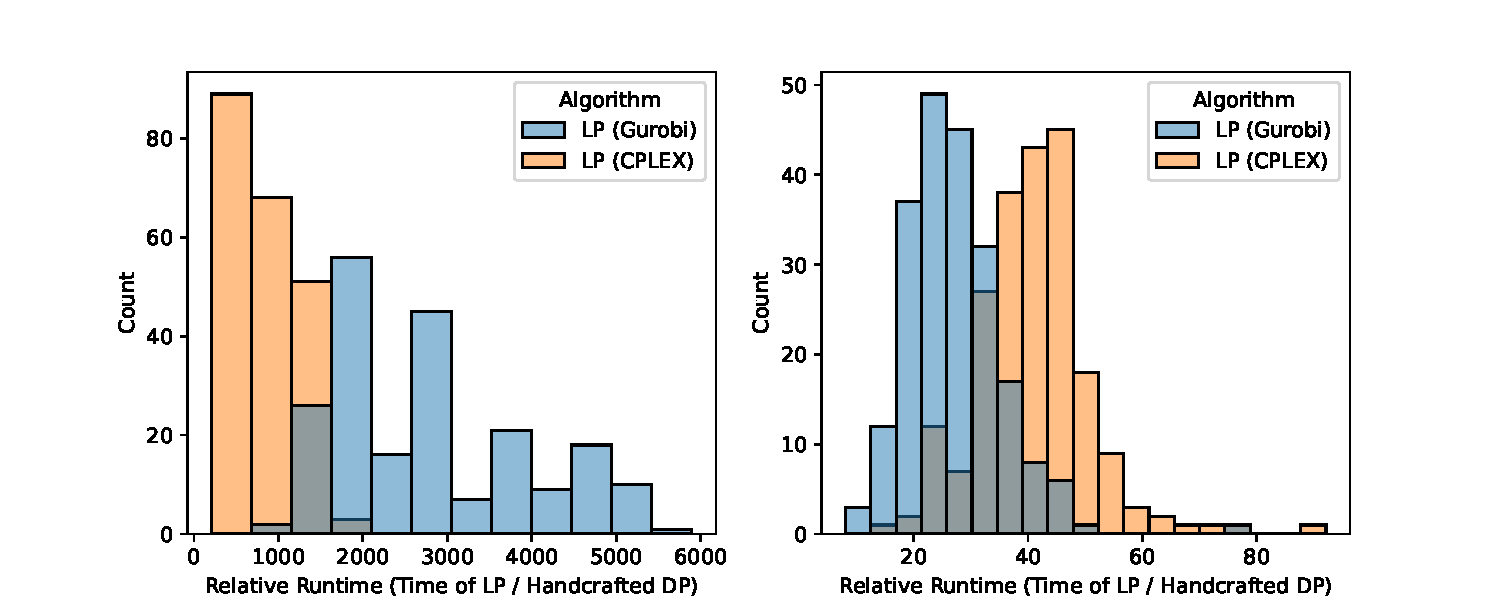
\includegraphics[width=\textwidth]{figures/sim_timing_relative_speedup.pdf}
    \caption{
        \label{fig:sim_timing_relative_speedup}
        Relative wall-clock runtime comparison of our algorithm to that of two commercial linear programming solvers, 
        Gurobi and CPLEX. \textbf{(Left)} The comparison includes both the time to build and solve the model. 
        \textbf{(Right)} The comparison includes only the time to solve the model.
    }
\end{figure}

To empirically demonstrate the utility of our regression algorithm, we compared an
implementation of our algorithm to a linear programming (LP) based approach.
In particular, we implemented the natural primal and dual LP formulations solving the VAF 
$\ell_1$ regression problem (Supplementary Section \henri{ref}) using two 
commercial LP solvers, Gurobi \cite{gurobi} and CPLEX \cite{ibm_cplex}. Then, we simulated
264 pairs of frequency matrices $F$ and clonal matrices $B$, and measured
the wall-clock runtime of our algorithm and the LP solvers on these simulated instances (Supplementary Section \henri{ref}). 
When measuring the runtime of the LP solvers, we separated the 
time required to solve the LP and the time required to construct the LP. Including only the
time solve the model, we found that our algorithm was a median of $26.5$ times faster than Gurobi and 
$41.2$ times faster than CPLEX (Figure \ref{fig:sim_timing_relative_speedup}). 
When considering both the time required to build and to solve the LP, our algorithm was a median of $2676.0$ times faster than Gurobi 
and $875.9$ times faster than CPLEX (Figure \ref{fig:sim_timing_relative_speedup}). 

\subsection{Evaluation on simulated data}
\begin{figure}
    \centering
    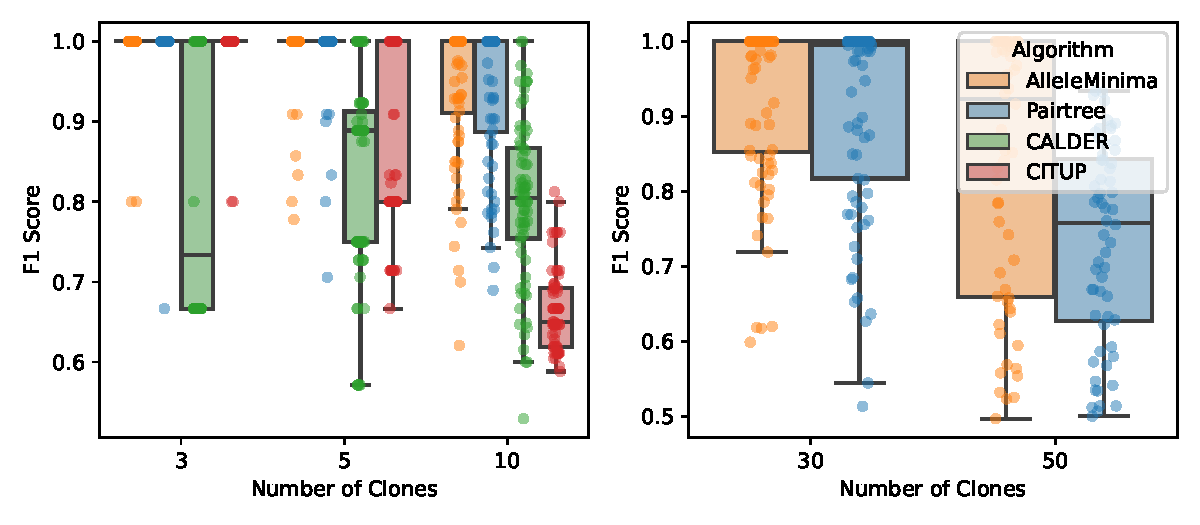
\includegraphics[width=\textwidth]{figures/sim_f1_score.pdf}
    \caption{
        \label{fig:sim_f1_score}
        The accuracy of reconstructing pairwise relations \ourmethod, CITUP \cite{malikic_clonality_2015}, 
        CALDER \cite{myers_calder_2019}, and Pairtree \cite{wintersinger_reconstructing_2022} on simulated data. 
        \textbf{(Left)} The F1-score of on 
        instances with $\leq 10$ clones. \textbf{(Right)} The F1-score on instances with 
        $> 20$ clones, methods that did not scale to these instances were excluded.
    }
\end{figure}

\newpage
\bibliographystyle{plain}
\bibliography{references}

\newpage
\appendix
\section{Supplementary Proofs}
\label{sec:supplementary_proofs}
\clonallycanonical*
\begin{proof}
    Suppose the theorem holds for all $k < n$. Clearly, the theorem holds for the base case when $n = 1$.

    $(i) \Rightarrow (ii)$: Let $\tree$ be the $n$-clonal tree associated with $\tree$. Consider a 
    relabeling of the clones of $\tree$ by their preorder traversal index during a breadth first search
    of $\tree$ starting at the root. Then, $r(\tree)$ is assigned index $1$ and the children of $r(\tree)$ 
    are assigned indices $2, \ldots, k + 1$ where $k$ is the number of children of $r(\tree)$. Let $B'$
    be the clonal matrix associated with $\tree$ under this relabeling. Then, $B'_{i,1} = 1$
    and $B'_{1, j} = 0$ for all $j \in \{2, \ldots, n\}$ since all clones contains the mutation $1$ 
    and the root only contains the mutation $1$. Let $B_1, \ldots, B_k$ be defined recursively
    as the clonally canonical matrices associated with the subtrees rooted at the children of $r(\tree)$,
    which exist by the inductive hypothesis. Then, $B'$ is clonally canonical with blocks $B_1, \ldots, B_k$,
    completing this direction of the proof.

    $(ii) \Rightarrow (i)$: Let $\tree_1, \ldots, \tree_k$ be the clonal trees associated with the
    clonally canonical matrices $B_1, \ldots, B_k$ of $B_{2:n, 2:n}$, respectively. These 
    are guaranteed to exist by the inductive hypothesis. Then, the clonal 
    tree $\tree$ associated with $B$ is the tree with root $1$ and children $2, \ldots, k + 1$ obtained
    by attaching the roots of $\tree_1, \ldots, \tree_k$ to the root of $\tree$. This completes
    this direction of the proof.

    The equivalence of $(i)$ and $(iii)$ follows from Lemma 1 of \cite{el-kebir_reconstruction_2015},
    this completes the proof.
\end{proof}


\hform*
\begin{proof}
    If $i^* = \infty$, all slopes $s_i$ are non-negative and the function $g(\psi')$ is non-decreasing.
    Thus, the maximum of $g(\psi')$ over any interval $[\psi - 1, \psi + 1]$, is achieved at the interval's right
    most value $\psi + 1$. 

    If $i^* = -\infty$, all slopes $s_i$ are negative and the function $g(\psi')$ is strictly decreasing. 
    Thus, the maximum of $g(\psi')$ over any interval $[\psi - 1, \psi + 1]$, is achieved at the interval's left
    most value $\psi - 1$. However, since $\psi'$ is constrained to be non-negative, if $\psi < 1$ the maximum
    is achieved at $\psi' = 0$.

    If $i^* \neq \infty, -\infty$, then $g(\psi')$ is non-decreasing on the interval $[0, i^*]$ and non-increasing
    on the interval $[i^*, \infty)$. Further, the maximum of $g(\psi')$ over all non-negative $\psi'$ is bounded
    and equal to $g(i^*)$. The result then follows by a case analysis on the value of $\psi$. If $\psi$ is in $[i^* - 1, i^* + 1]$, then
    we can take $\psi' = i^*$ and achieve the maximum. If $\psi < i^* - 1$, then the function $g(\psi')$ is non-decreasing 
    on the interval $[\psi - 1, \psi + 1]$ and the maximum is achieved at the interval's right most value $\psi + 1$. 
    Symetrically, if $\psi > i^* + 1$, then the function $g(\psi')$ is non-increasing on the interval $[\psi - 1, \psi + 1]$ and the 
    maximum is achieved at the interval's left most value $\psi - 1$, which is always non-negative since $\psi > 1$. 
    As this covers all possible cases, this proves that $h$ has the form \eqref{eq:h_form}.

    To see that $h(\psi)$ is continuous, observe that
    \[\lim_{\psi \to (i^* - 1)^-} h(\psi) = g(i^*) \quad\text{and}\quad \lim_{\psi \to (i^* + 1)^+} h(\psi) = g(i^*)\]
    at the only candidates for discontinuity, $i^* - 1$ and $i^* + 1$. To see that it is concave, note that
    \[h''(\psi) = \begin{cases}
        \,0 &\text{if } \psi \in [i^* - 1, i^* + 1],\\
        \,g''(\psi + 1) &\text{if } \psi < i^* - 1,\\
        \,g''(\psi - 1) &\text{if } \psi > i^* + 1.
    \end{cases}\]
    As $g(\psi)$ is concave, its second derivative $g''(\psi)$ is non-positive, which implies that $h(\psi)$ is also concave. Since $h$ is trivially
    piecewise linear by \eqref{eq:h_form}, the proof is complete.
\end{proof}


\end{document}
